\documentclass[main.tex]{subfiles}

\begin{document}

\section{Exploratívna analýza}
V exploratívnej analýze sme sa zamerali na ukázanie relevantnosti dát, ktoré sme nazbierali a rovnako aj na vytvorenie si očakávaní od predikčného modelu. Teda po nazbieraní a uprataní dát sme hlavne riešili to, ako dané dáta budeme kombinovať a či niektoré z nich budú relevantné pre náš predikčný model.

\subsection{Náhľad do dát polls_by_election}
Hlavný dataset obsahuje dáta, ktorú máme v plane v upravenej verzi použiť na predikciu volebných výsledkov. Pre každú stranu dataset obsahuje posledných 12 prieskumov a výsledky volieb spolu s informáciami, či bola strana v parlamente, opozícii, alebo koalícii. Bolo by teda vhodné sa pozrieť na to ako sa vyvijali volebné prieskumy 12 mesiacov pred voľbami. Ak by sme našli jasne trendy kedy strana postupne rastie v čase chceli by sme očakávať od nášho modelu, že tento rast sa v ňom ukáže. 

Teda na ukážku sme si vybrali dáta z minulo ročných volieb a rovnako sme vyfiltrovali strany čo dosiahly v prieskumoch pred voľbami nenulový výsledok. 
\begin{figure}[!htbp]
    \centering
    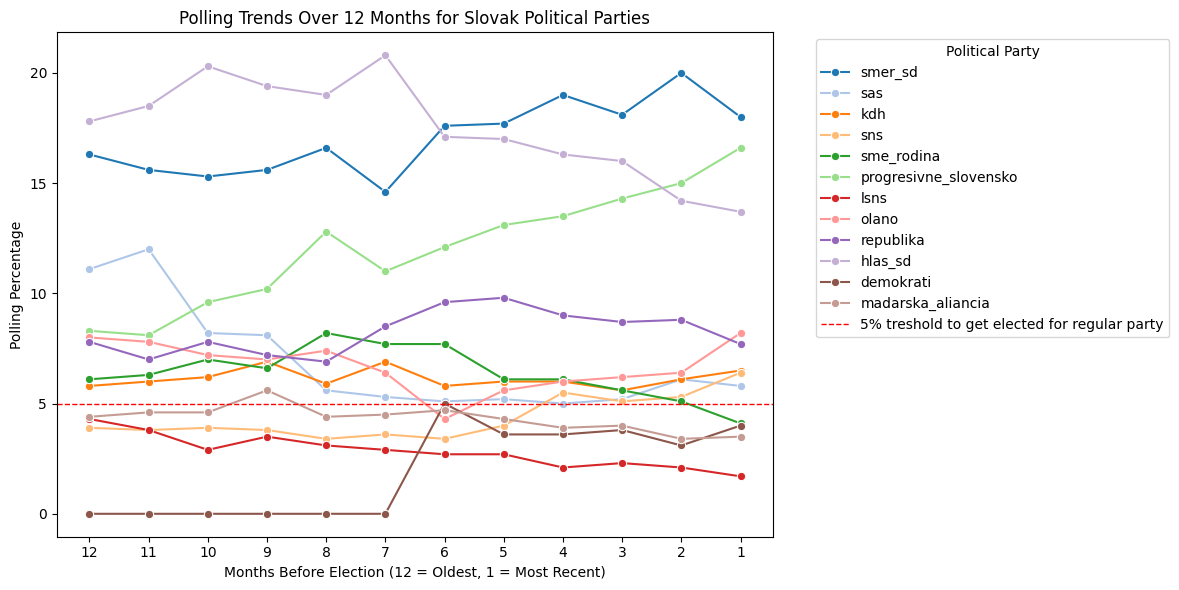
\includegraphics[width=\textwidth]{../images_exploratory/Polls_without_result_2023.png}
    \caption{}
    \label{fig:example}
\end{figure}

Už môžeme pozorovať ako sa vyvíjali názori voličov pred voľbami, napriklad zrod strany Demokrati alebo postupný prepad Hlasu či postupný nárast Progresivneho Slovenska.
Pridanie výsledku vo voľbách by malo ešte väčšiu výpovednú hodnotu, keďže budeme vedieť zhodnotiť aj to ako sa preferencie premietli už aj vo voľbách, a tak urobime presne to.
\begin{figure}[!htbp]
    \centering
    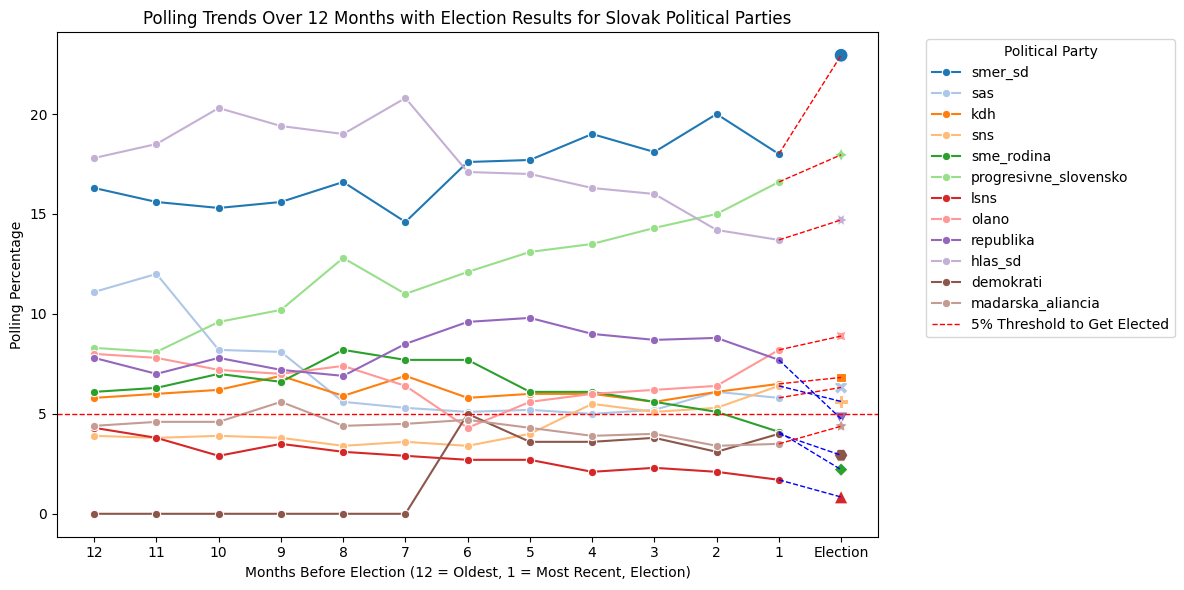
\includegraphics[width=\textwidth]{../images_exploratory/Polls_with_result_2023.png}
    \caption{}
    \label{fig:example}
\end{figure}

Je jasne, že prieskumy zachytavajú realitu pred voľbami relatívne dobre aj keď vidíme aj značné skoky pre určite strany. Avšak poradie toho ako strany dopadli vo voľbách sa skoro nezmenilo až na výrazný prepad strany Republika.
Vidíme aj, že trendy v prieskumoch maju vplyv na to ako strana dopadne vo voľbách ale aj tu sa nájdu vynimky ako Hlas, ktorý niekoľko mesiacov pred voĺbami padal ale nakoniec dopadol lepšie ako v posledných prieskumoch. Taktiež ak sa niektoré strany dostali až pod hranicu zvoliteľnosti v prieskumoch často ju už neprekonali. Voliči majú prirodzený strach, že im prepadne hlas, a tak práve takýto výsledok v prieskumoch môže veľmi ubližiť strane.

Toto bol pohľad len na najnedávnejšie voľby, ale ako vyzerali aj tie predtým?

\clearpage


\begin{figure}[!htbp]
    \centering
    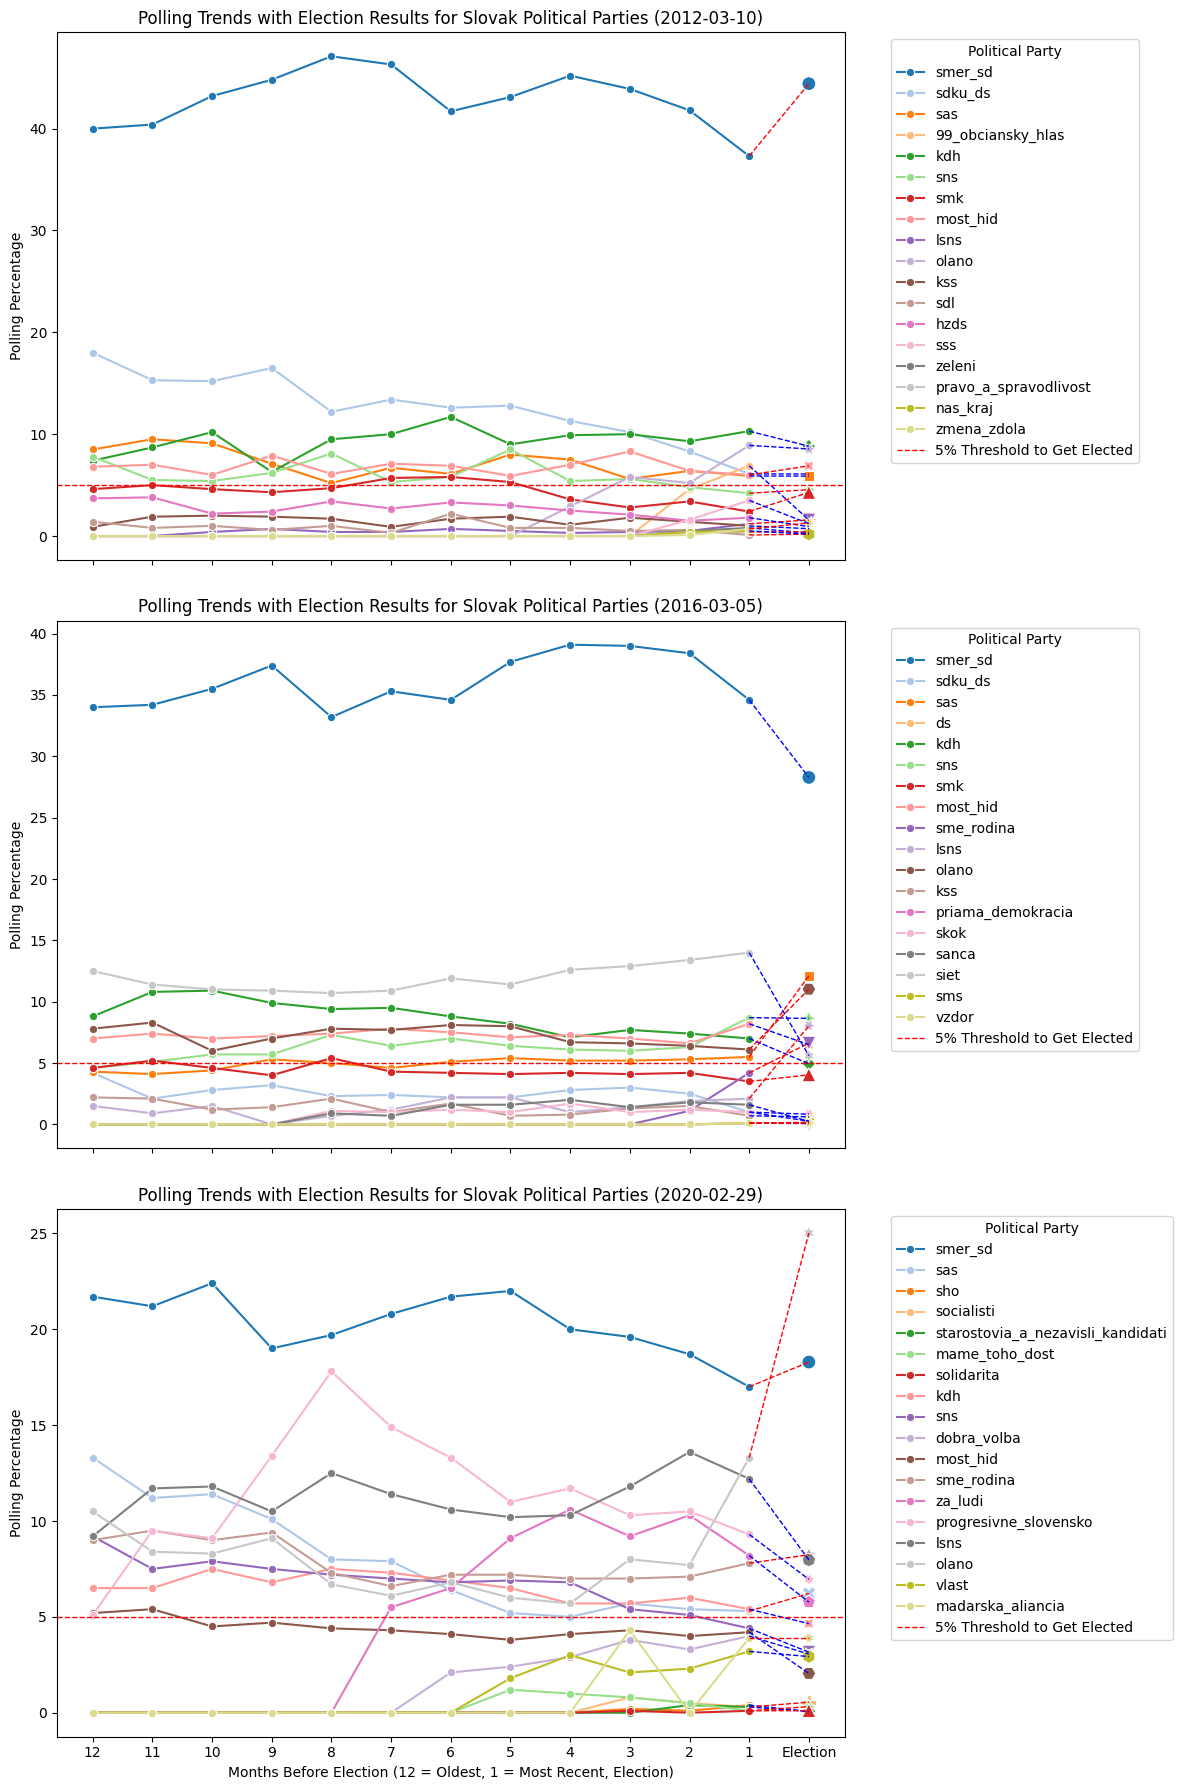
\includegraphics[width=\textwidth]{../images_exploratory/Polls_with_result_ALL.png}
    \caption{}
    \label{fig:example}
\end{figure}

Voľby v roku 2012 mali jasného favorita v strane Smer, ktorá po voľbách aj sama zostavila vládu, za nasledok čoho sa považuje chaotický pád vlady a následné predčasné voľby. Strana sdku sa dramaticky prepadala v prieskumoch z 18 percent rok pred voľbami až na 6 percent v voľbách. 

V voľbách roku 2016 už Smer stratil na sile a v posledných mesiacoch kampane utrpel prepad na 28 percent. Zaujimavý vývoj mala strana Sieť, ktorá v prieskumoch obdržavala na 10 percent avšak v poslednom mesiaci kampane jej voliči pravdepodobne prestúpili k iným stranám ako Oľano, SAS či Sme rodina. Sieť sa tak prepadla až na hranicu zvoliteľnosti 5tich percent.

Voľby v roku 2020 sa ukazujú ako najvyrovnanejšie a to v tom zmysle, že viac strán dosahovalo v prieskumoch nad hranicu 10 percent. Avšak ujať vedenia sa podarilo strane Oĺano, ktorá rástla exponencialne v posledných mesiacoch pred voĺbami až ich aj nakoniec vyhrala. Graf nezachytáva realitu, toho že strane Progresivne Slovensko-Spolu sa nedostalo do parlamentu, keďže kandidovali ako koalicia dvoch stán a pre takýto typ politického objektu je potrebné dosiahnuť vo voľbach viac ako 7 percent. 

Trend toho, že vládne strany počas výkonnu moci strácajú na podpore v následujúcich voľbach vyzerá ustálený v ramci všetkých volieb, ešte sa naň pozrieme bližšie. 

\subsection{Dopad predošleho vládnutia na voľby}

V našich dátach je informácia o tom či v predošlom volebnom období bola daná strana súčasťou koalicie alebo bola v parlamente/opozicií. Bolo by teda vhodne sa pozrieť na to ako sa hýbali voličske zakladne od strán v koalicíi a strán ktoré v nej neboli. 
\begin{figure}[!htbp]
    \centering
    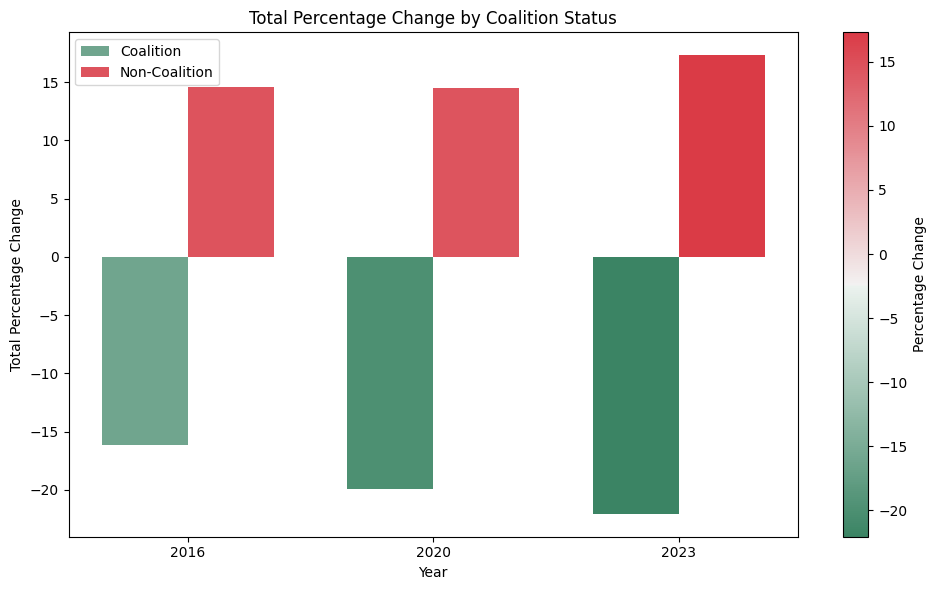
\includegraphics[width=\textwidth]{../images_exploratory/Coalition_vs_NoCoalition.png}
    \caption{}
    \label{fig:example}
\end{figure}

V súčte strany vládnej moci vždy stratili až cez 15 percent v následujúcich voľbách avšak miera straty nebola ustálená, teda chceme veriť, že kvalita vládnutia aspoň do nijakej miery ovplyvnila koľko by dané strany stratili v následujúcich voľbách.
V závislosti od tohto strany mimo vladnej koalicie nabrali vo výsledkoch zhruba v rovnakom množstve. 

\end{document}
